\documentclass{standalone}
\begin{document}
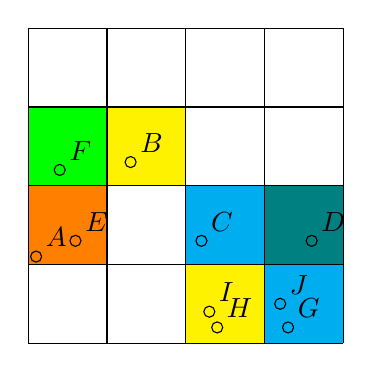
\begin{tikzpicture}

\fill[orange] (0, 1) rectangle (1, 2);
\fill[cyan] (2, 1) rectangle (3, 2);
\fill[cyan] (3, 0) rectangle (4, 1);
\fill[green] (0, 2) rectangle (1, 3);
\fill[yellow] (2, 0) rectangle (3, 1);
\fill[yellow] (1, 2) rectangle (2, 3);
\fill[teal] (3, 1) rectangle (4, 2);

\draw (0, 0) -- (0, 4);
\draw (1, 0) -- (1, 4);
\draw (2, 0) -- (2, 4);
\draw (3, 0) -- (3, 4);
\draw (4, 0) -- (4, 4);

\draw (0, 0) -- (4, 0);
\draw (0, 1) -- (4, 1);
\draw (0, 2) -- (4, 2);
\draw (0, 3) -- (4, 3);
\draw (0, 4) -- (4, 4);

\draw (.1, 1.1) circle (2pt) node[above right] {$A$};
\draw (1.3, 2.3) circle (2pt) node[above right] {$B$};
\draw (2.2, 1.3) circle (2pt) node[above right] {$C$};
\draw (3.6, 1.3) circle (2pt) node[above right] {$D$};
\draw (.6, 1.3) circle (2pt) node[above right] {$E$};

\draw (.4, 2.2) circle (2pt) node[above right] {$F$};
\draw (3.3, .2) circle (2pt) node[above right] {$G$};
\draw (2.4, .2) circle (2pt) node[above right] {$H$};
\draw (2.3, .4) circle (2pt) node[above right] {$I$};
\draw (3.2, .5) circle (2pt) node[above right] {$J$};


\end{tikzpicture}
\end{document}
